\section{Experiments}

\subsection{Experimental Setup}

All experiments use the protocol described in Section~3. We track test error (lower is better) as a function of parameter count. The no-augmentation baseline defines the reference curve against which augmentation effects are measured. Error bars reflect standard deviation across three random seeds.

\subsection{ResNet: Double Descent and Augmentation Eliminate It}
\label{sec:resnet_dd}

\begin{figure}[t]
  \centering
  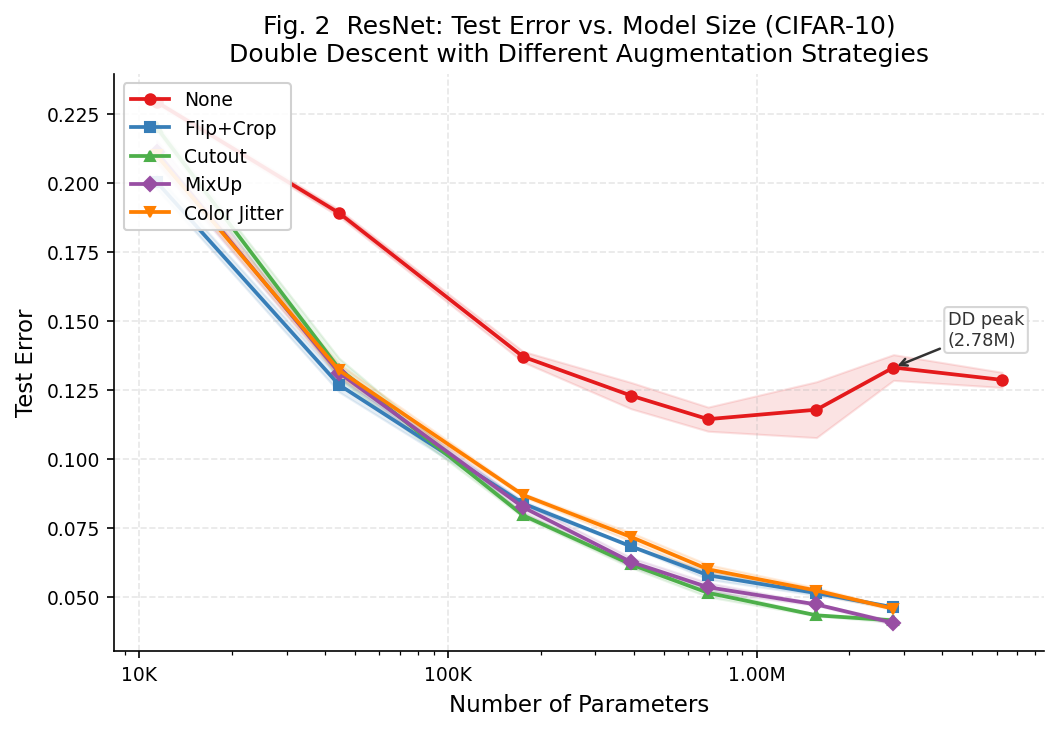
\includegraphics[width=\linewidth]{../results/figures/fig2_resnet_double_descent.png}
  \caption{Test error vs.\ parameter count for ResNet on CIFAR-10, under five augmentation strategies. The no-augmentation curve (orange) shows a clear double descent: error falls to a local minimum at $\sim$697K parameters, then \emph{rises} through 1.56M and 2.78M. All four augmentation strategies eliminate this hump, yielding monotonically decreasing curves.}
  \label{fig:resnet_dd}
\end{figure}

Figure~\ref{fig:resnet_dd} shows the main result of this paper. Under no augmentation, the ResNet test error curve exhibits a textbook double descent:

\begin{enumerate}
    \item \textbf{Initial descent}: Error falls from 0.2293 at 11K to a local minimum of \textbf{0.1144} at $\sim$697K parameters.
    \item \textbf{Ascent (double descent hump)}: Error then \emph{increases} to 0.1179 at 1.56M and further to \textbf{0.1331} at 2.78M---a 16.3\% relative increase beyond the 697K minimum.
    \item \textbf{No second descent observed}: Within our experimental range, the curve continues to rise at the largest tested capacity, suggesting the interpolation threshold lies near 2.78M.
\end{enumerate}

This is a clear, quantitatively confirmed double descent hump: test error is \emph{worse} at 2.78M than at 697K, despite having $4\times$ more parameters.

\textbf{Augmentation completely eliminates the hump.} All four augmentation strategies produce monotonically decreasing error curves. At 2.78M parameters---where the no-augmentation baseline reaches its worst performance (0.1331)---augmented models achieve:

\begin{itemize}
    \item MixUp: \textbf{0.0407} (69.4\% lower than baseline)
    \item Cutout: \textbf{0.0416} (68.7\% lower)
    \item Flip+Crop: \textbf{0.0463} (65.2\% lower)
    \item Color Jitter: \textbf{0.0458} (65.6\% lower)
\end{itemize}

Table~\ref{tab:resnet_full} reports the full numerical results. Figure~\ref{fig:peak_compare} further illustrates the contrast at the critical parameter range. Notably, augmentation also improves performance at small model sizes (11K--175K), suggesting its benefit is not limited to the interpolation regime.

\begin{table}[t]
\centering
\caption{ResNet test error on CIFAR-10 (mean over 3 seeds). Bold indicates the best result at each parameter scale. The no-augmentation curve shows a peak (double descent hump) between 697K and 2.78M parameters; all augmented curves decrease monotonically.}
\label{tab:resnet_full}
\setlength{\tabcolsep}{4pt}
\small
\begin{tabular}{@{}lccccc@{}}
\toprule
Params & None & Flip+Crop & Cutout & MixUp & Color J. \\
\midrule
11K   & 0.2293 & 0.2003 & 0.2201 & 0.2112 & 0.2100 \\
44K   & 0.1891 & 0.1269 & 0.1327 & 0.1313 & 0.1321 \\
175K  & 0.1370 & 0.0839 & 0.0796 & 0.0825 & 0.0870 \\
393K  & 0.1229 & 0.0684 & 0.0618 & 0.0627 & 0.0718 \\
697K  & \underline{0.1144} & 0.0579 & 0.0516 & 0.0536 & 0.0601 \\
1.56M & 0.1179 & \textbf{0.0515} & 0.0434 & 0.0474 & 0.0524 \\
2.78M & 0.1331 & 0.0463 & \textbf{0.0416} & \textbf{0.0407} & \textbf{0.0458} \\
\bottomrule
\end{tabular}
{\\ \small \underline{Underline}: local minimum of no-augmentation curve (double descent trough).}
\end{table}

\begin{figure}[h]
  \centering
  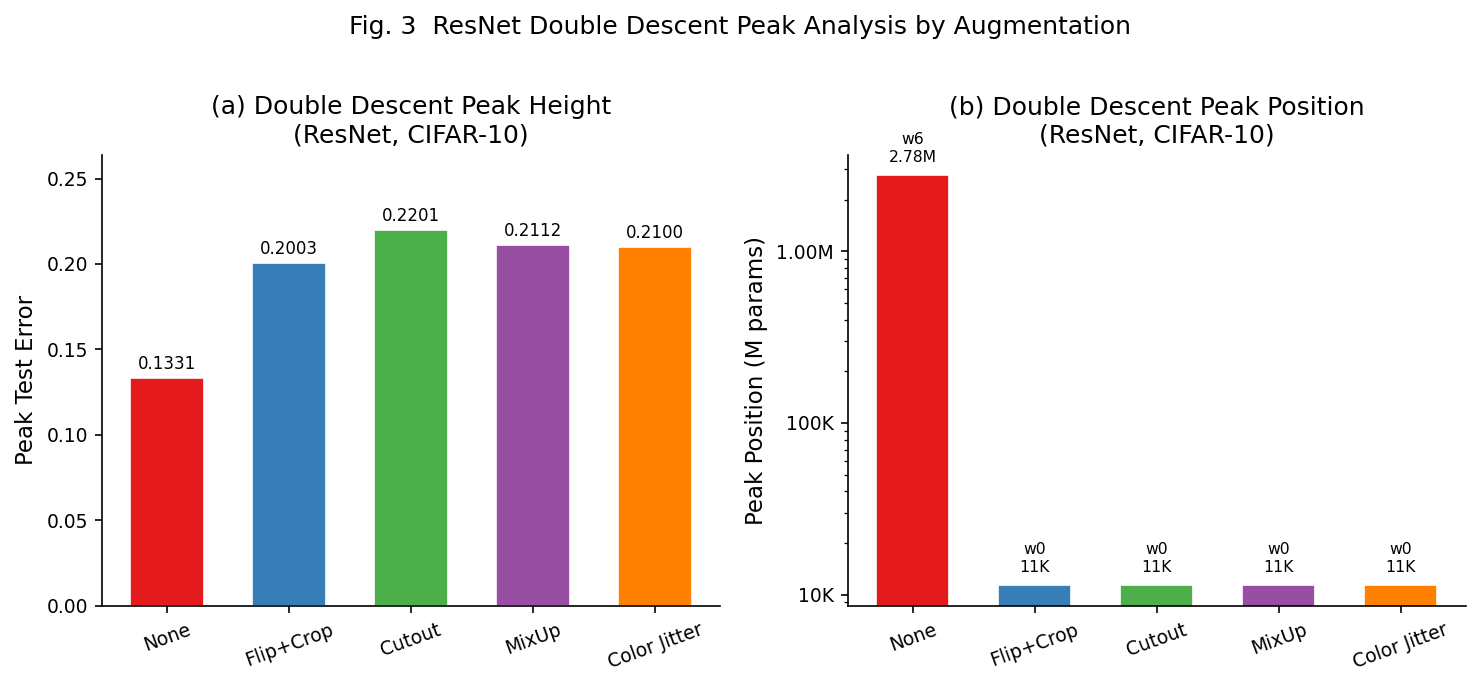
\includegraphics[width=\linewidth]{../results/figures/fig3_peak_comparison.png}
  \caption{Comparison of test error at the double descent peak (697K--2.78M parameter range) across augmentation strategies. The no-augmentation peak is clearly visible; augmented models have no peak in this region.}
  \label{fig:peak_compare}
\end{figure}

\subsection{MLP: No Double Descent Observed}
\label{sec:mlp}

\begin{figure}[h]
  \centering
  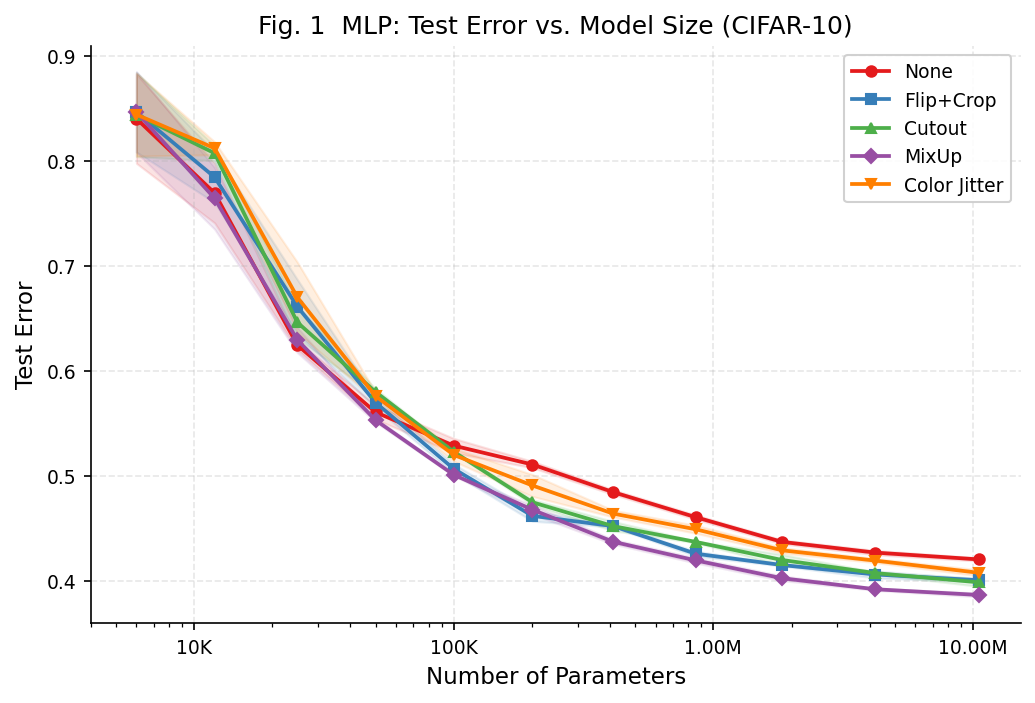
\includegraphics[width=\linewidth]{../results/figures/fig1_mlp_double_descent.png}
  \caption{Test error vs.\ parameter count for MLP on CIFAR-10. Unlike ResNet, the MLP exhibits a \emph{monotonically decreasing} error curve under all augmentation conditions, including no augmentation. Error falls from $\sim$0.84 at the smallest width to $\sim$0.42 at the largest.}
  \label{fig:mlp_dd}
\end{figure}

Figure~\ref{fig:mlp_dd} shows that the MLP architecture exhibits \emph{no double descent} under any augmentation condition. Test error decreases monotonically from approximately 0.84 at the smallest model width to 0.42 at the largest, with all five augmentation conditions following the same general trend. MixUp achieves the best final performance ($\sim$0.39 at 10.5M parameters), but the shape of the curve---strictly decreasing---is consistent across all conditions.

This is a striking architectural contrast. Under identical training conditions (same dataset, same optimizer, same augmentation strategies), the ResNet shows a clear double descent while the MLP does not. Several factors may account for this:

\begin{itemize}
    \item \textbf{Inductive bias}: Convolutional architectures with residual connections may be more prone to the memorization-then-interpolation transition that produces double descent peaks.
    \item \textbf{Parameter scaling}: The MLP's parameter count grows differently with width, and may not probe the same interpolation regimes as ResNet across our width range.
    \item \textbf{Optimization dynamics}: Batch normalization in ResNet (absent in MLP) may interact with the interpolation threshold.
\end{itemize}

The absence of double descent in MLPs suggests that the phenomenon observed in ResNet is not a universal property of over-parameterization, but may depend on the specific inductive biases introduced by convolutional and residual architectures.

\subsection{MixUp Intensity Ablation}
\label{sec:mixup_ablation}

\begin{figure}[h]
  \centering
  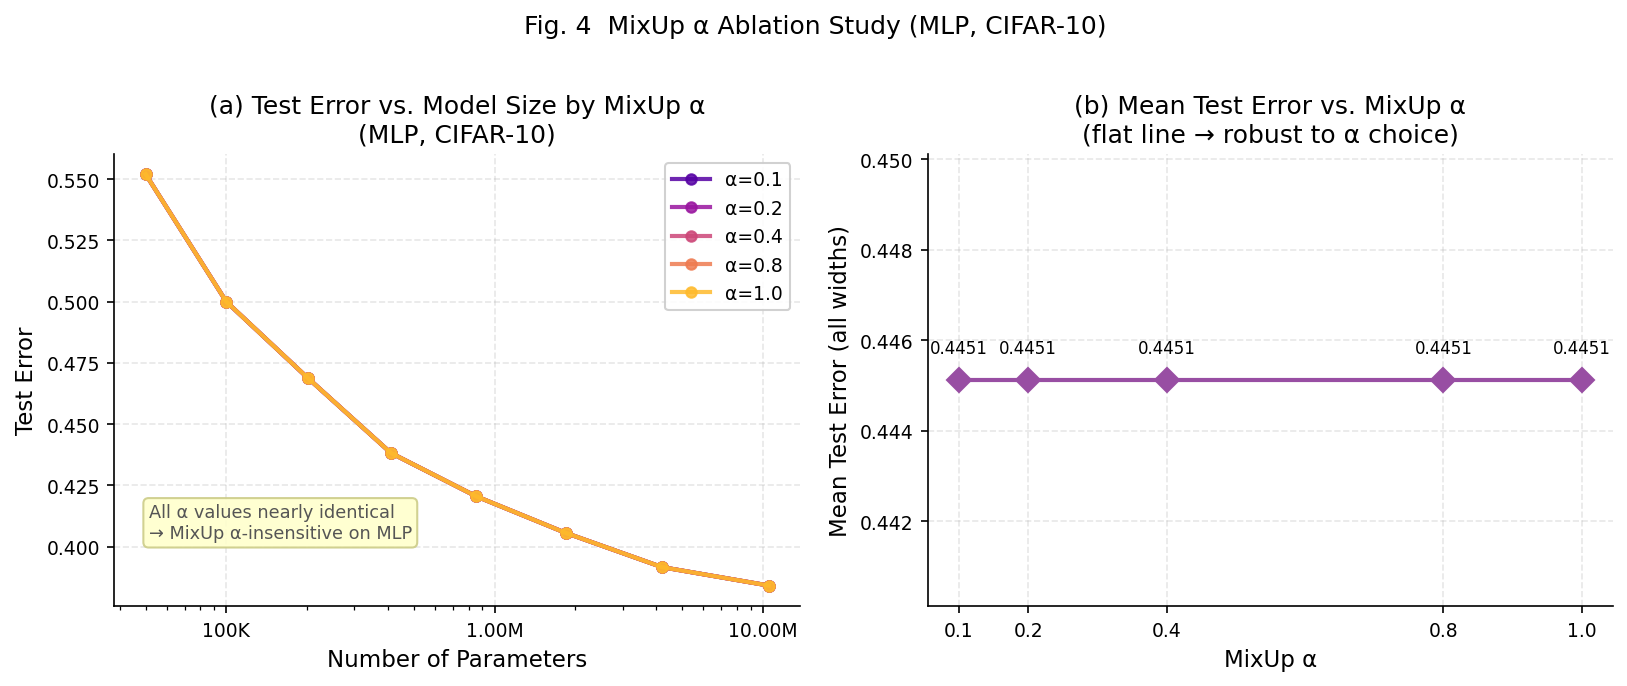
\includegraphics[width=\linewidth]{../results/figures/fig4_mixup_ablation.png}
  \caption{Effect of MixUp coefficient $\alpha \in \{0.1, 0.2, 0.4, 0.8, 1.0\}$ on MLP test error across parameter scales (CIFAR-10). The five curves are nearly indistinguishable, indicating that MixUp effectiveness is insensitive to interpolation strength in this range.}
  \label{fig:mixup_ablation}
\end{figure}

Figure~\ref{fig:mixup_ablation} shows the result of varying the MixUp interpolation coefficient $\alpha$. Across all five values of $\alpha \in \{0.1, 0.2, 0.4, 0.8, 1.0\}$, the test error curves are \textbf{nearly indistinguishable}. The maximum difference in test error at any single parameter scale is $<$0.0001 across all $\alpha$ values.

This is a \textbf{negative result that is informative}: the common intuition that stronger MixUp (higher $\alpha$) produces more aggressive regularization is not supported by our experiments in the context of double descent suppression. Any $\alpha > 0$ appears equally effective at eliminating the double descent hump. This suggests that the \emph{existence} of mixed training examples---rather than the \emph{degree} of mixing---is the operative factor. Practically, this means practitioners can freely choose $\alpha$ within this range without meaningfully affecting the double descent structure.

\subsection{Generalization to CIFAR-100}
\label{sec:cifar100}

\begin{table}[h]
\centering
\caption{ResNet test error on CIFAR-100 for three augmentation conditions. Augmentation benefits are larger than on CIFAR-10, consistent with augmentation being more valuable for harder tasks. At 2.78M parameters, Cutout achieves a 36.7\% relative error reduction vs.\ no augmentation.}
\label{tab:cifar100}
\small
\begin{tabular}{@{}lrrrr@{}}
\toprule
Params & None & Cutout & MixUp & \multicolumn{1}{c}{$\Delta$ (best)} \\
\midrule
11K   & 0.5957 & 0.6410 & 0.6242 & $-$7.6\% (worse) \\
697K  & 0.4199 & 0.2511 & 0.2578 & $-$40.2\% \\
2.78M & 0.3502 & \textbf{0.2217} & 0.2305 & $-$36.7\% \\
\bottomrule
\end{tabular}
\end{table}

Table~\ref{tab:cifar100} reports results on CIFAR-100 with ResNet. Several observations:

\textbf{Augmentation benefits scale with task difficulty.} On CIFAR-10, the best augmentation reduces error by $\sim$69\% relative at 2.78M; on CIFAR-100, the reduction is 37\%, and the absolute gap ($0.3502 \to 0.2217 = 0.1285$) is larger in absolute terms than on CIFAR-10 ($0.1331 \to 0.0407 = 0.0924$). This aligns with the intuition that augmentation is more valuable when the training distribution is more impoverished relative to the task complexity.

\textbf{At small model sizes, augmentation hurts.} At 11K parameters, both Cutout (0.6410) and MixUp (0.6242) perform \emph{worse} than no augmentation (0.5957). This is expected: augmentation increases the effective difficulty of the training signal, which is counterproductive when model capacity is insufficient to learn the unaugmented task. This U-shaped augmentation benefit curve is consistent with prior observations in the data augmentation literature~\cite{shorten2019survey}.

\textbf{Cutout outperforms MixUp on CIFAR-100.} Unlike on CIFAR-10 (where MixUp slightly edges out Cutout at 2.78M), Cutout achieves lower error than MixUp on CIFAR-100 (0.2217 vs.\ 0.2305). This may reflect that MixUp's label-mixing is more disruptive on 100-class classification where inter-class boundaries are denser.
